\section{The Full Spatial Readout Comparison}
\label{app:readout}

How much of a point-hit score comes from the way a location is requested and
parsed? The readout experiment crosses pixel and normalized-1000 requests with
JSON and two-line text. Table~\ref{tab:protocol-full} retains every query in the
denominator and reports numeric-output coverage beside end-to-end hits. A
parsed point contributes to coverage even if it is outside the image; a hit
must also lie inside the image and target box.

In the text condition, the prompt requests \texttt{Point: x, y} followed by
\texttt{Answer: target category}. JSON requests \texttt{point\_xy} and
\texttt{answer}. Because the category is supplied in the prompt, repeating it
measures answer adherence, not independent recognition. The clean two-view
prompt requests only a point.

\begin{table}[htbp]
\centering\small
\setlength{\tabcolsep}{3pt}
% Generated by scripts/build_assets.py from corrected results.json
\begin{tabular}{lllrrrr}
\toprule
Model & Frame & Format & $V_O$ & $V_C$ & $H_O$ (\%) & $H_C$ (\%) \\
\midrule
Gemma4-E4B & 0--1000 & text & 30/30 & 30/30 & 90.0 & 96.7 \\
Gemma4-E4B & 0--1000 & JSON & 30/30 & 30/30 & 90.0 & 86.7 \\
Gemma4-E4B & pixel & text & 30/30 & 30/30 & 36.7 & 36.7 \\
Gemma4-E4B & pixel & JSON & 30/30 & 30/30 & 0.0 & 0.0 \\
Qwen2.5-VL-7B & 0--1000 & text & 29/30 & 29/30 & 10.0 & 13.3 \\
Qwen2.5-VL-7B & 0--1000 & JSON & 9/30 & 12/30 & 13.3 & 6.7 \\
Qwen2.5-VL-7B & pixel & text & 26/30 & 25/30 & 80.0 & 66.7 \\
Qwen2.5-VL-7B & pixel & JSON & 18/30 & 22/30 & 60.0 & 73.3 \\
Qwen3-VL-2B & 0--1000 & text & 30/30 & 30/30 & 86.7 & 86.7 \\
Qwen3-VL-2B & 0--1000 & JSON & 30/30 & 30/30 & 90.0 & 93.3 \\
Qwen3-VL-2B & pixel & text & 30/30 & 30/30 & 60.0 & 60.0 \\
Qwen3-VL-2B & pixel & JSON & 30/30 & 30/30 & 0.0 & 0.0 \\
Qwen3-VL-8B & 0--1000 & text & 30/30 & 30/30 & 93.3 & 96.7 \\
Qwen3-VL-8B & 0--1000 & JSON & 30/30 & 30/30 & 93.3 & 96.7 \\
Qwen3-VL-8B & pixel & text & 30/30 & 30/30 & 0.0 & 3.3 \\
Qwen3-VL-8B & pixel & JSON & 30/30 & 30/30 & 0.0 & 0.0 \\
InternVL3-8B & 0--1000 & text & 25/30 & 26/30 & 60.0 & 66.7 \\
InternVL3-8B & 0--1000 & JSON & 11/30 & 7/30 & 36.7 & 20.0 \\
InternVL3-8B & pixel & text & 30/30 & 29/30 & 16.7 & 10.0 \\
InternVL3-8B & pixel & JSON & 11/30 & 16/30 & 10.0 & 20.0 \\
Molmo-7B-D & 0--1000 & text & 30/30 & 30/30 & 90.0 & 96.7 \\
Molmo-7B-D & 0--1000 & JSON & 30/30 & 30/30 & 13.3 & 3.3 \\
Molmo-7B-D & pixel & text & 30/30 & 30/30 & 0.0 & 0.0 \\
Molmo-7B-D & pixel & JSON & 30/30 & 30/30 & 0.0 & 0.0 \\
\bottomrule
\end{tabular}

\caption{Full readout matrix. $V$ counts parsed numeric points among 30 queries;
$H$ is the end-to-end hit percentage over the same 30 queries. The normalized
text rows are exact-ID subsets of the current 80-pair runs; the other rows use
their recorded 30-pair runs.}
\label{tab:protocol-full}
\end{table}

For frame size $K$, $(u,v)$ maps to image pixels $(uW/K,vH/K)$. Pixel requests
use the point directly. Missing, malformed, and out-of-image points fail the
hit metric. The parser also handles historical four-number text lines by taking
the box center. Raw text remains available to distinguish an output-format
failure from a coordinate mismatch. A uniformly applied alternative frame is
reported as a diagnostic, rather than selected separately to fit each target.

The comparison reveals why both columns matter. A model can return numeric
points consistently yet locate the target poorly under the requested frame.
Conversely, low coverage can suppress end-to-end accuracy before localization
is assessed. A material difference measured through either interface therefore
needs the corresponding coverage and frame definition.

\subsection{Coordinate baselines}
The 30-pair target-centered archive admits a simple center solution: the image
center hits all 30 targets in both conditions when interpreted in pixels.
An oracle box center also hits all targets when expressed and scored in the
same frame. Interpreting either pixel baseline as normalized-1000 produces
zero hits in this set; expressing the oracle in normalized-1000 restores all
30 hits. These checks explain the move to two-view boards and verify that the
frame transformation is consequential even with identical numeric outputs.
A seeded random pixel baseline hits 5/30 original and 2/30 converted targets;
its normalized reinterpretation yields 8/30 and 3/30. These are scorer checks,
separate from model predictions.
Figure~\ref{fig:app-readout} follows a response through parsing and coordinate
interpretation before the point is scored.

\begin{figure}[htbp]
\centering
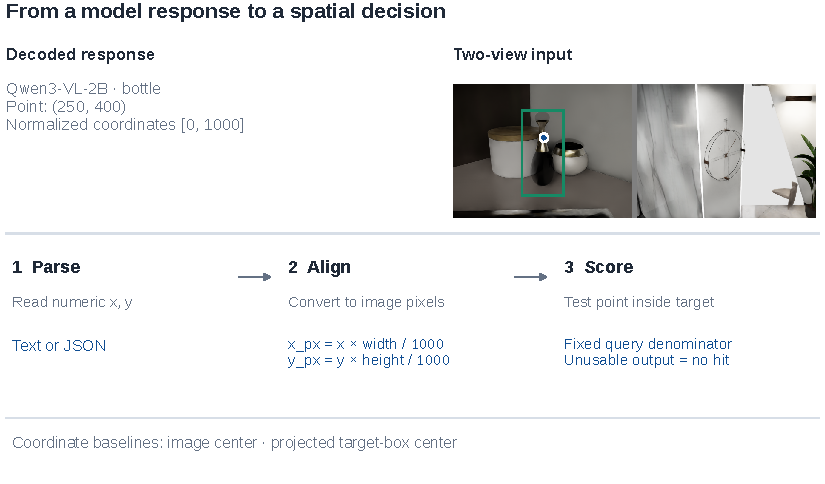
\includegraphics[width=\linewidth]{appendix_readout.pdf}
\caption{From a model response to a spatial score. Parsing establishes numeric
coverage; the requested coordinate frame places the point on the image, and
the target region determines a hit. Coordinate-only baselines expose the
effect of changing the interpretation of identical output numbers.}
\label{fig:app-readout}
\end{figure}
\FloatBarrier
